%% ----------------------------------------------------------------
%%? 2nd Draft Complete | TODO Missing Gantt Charts
%% ----------------------------------------------------------------
\chapter{Project Retrospective (1350 words)}
This chapter will go over the significant limitations and an improved ideal project plan.

%% ----------------------------------------------------------------
\section{Handling Complexity: Miro Mindmap}
%% ----------------------------------------------------------------
One of the major elements that significantly helped with planning the project and managing the complexity of the project was building a hierarchical mindmap in Miro (a highly flexible diagramming tool). The reason Miro's mindmap was useful was that it allowed for children nodes to be toggled, meaning that they were visually hidden, but still accessible.

This feature significantly helped in breaking down the mammoth complexity of the entire project. The project was decomposed into the high-level parts, getting more specific as the tree became deeper. These high-level parts can be seen in figure \ref{figure::miro::mindmap_high_level}. Expanded sections of this diagram can be found in appendix \ref{appendix::Miro}.
\begin{figure}
    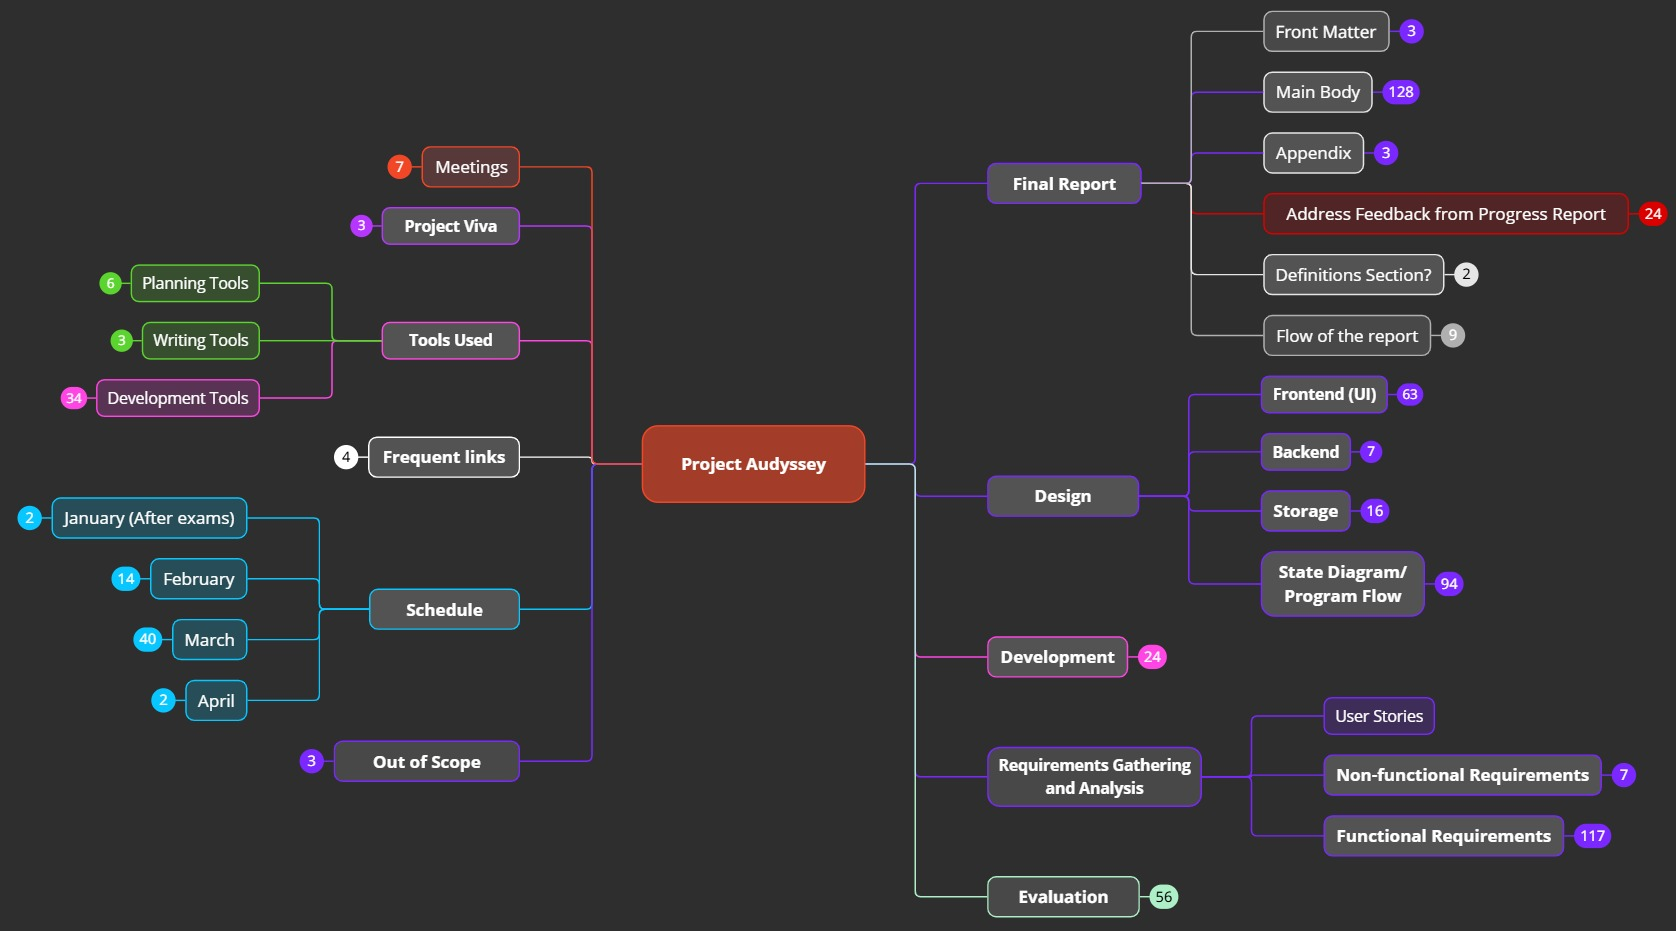
\includegraphics[angle=90, scale=0.43]{Miro_Mindmap_Depth_1,2}
    \caption{Miro Mindmap high level overview}
    \label{figure::miro::mindmap_high_level}
\end{figure}

The only issue with this diagram is the point at which it was used. This diagram was only built at the end of January meaning it was not helpful for the research and design stages, where it would have helped significantly.

%todo Do I add this because it doesn't reflect that well on me :(
The only drawback with this method is that whilst being able to hide child nodes is very useful, the count of hidden nodes is not that useful a metric. As such it was possible to hide nodes and forget about the contents which slightly hindered development.

%% ----------------------------------------------------------------
\section{Limitations}
%% ----------------------------------------------------------------
\subsection{Unfinished Code}
One of the key limitations of this project resides in the fact that the dynamic graph and audio journey features were not developed in time. This meant that these features were not able to be fully evaluated and therefore will require further research to truly understand them.

This is partly due to the unnecessary complexity in obtaining the Echo Nest attributes. The initial process to gain these attributes was through these endpoints via Spotify's API: \texttt{Get Track's Audio Features} and \texttt{Get Track's Audio Analysis}. However, as stated in \href{https://developer.spotify.com/blog/2024-11-27-changes-to-the-web-api}{this blog post}, these endpoints were deprecated.

As an alternative, I switched to using SoundCharts API to access the attributes. However, this API is paywalled and less precise but would still provide sufficient values for the graph views. Another issue with this workflow is that the complexity used up a lot of valuable development time. Had Exportify been found earlier, the project development phase would've been significantly smoother.

\subsubsection{Missed Opportunity to Reprioritise}
Whilst the SoundCharts workflow was unnecessarily complex, the other big issue is that the requirements should've been reprioritised. Whilst the static graphs provided a lot of insights as detailed in the evaluation, they were not the core focus of this project. Due to its novel nature, the dynamic graphs were more important and should've been re-prioritised once I realised that I would not have enough time to complete both graph views to a satisfactory standard.

The true/original niche/gap in the research was investigating better ways to create listening journeys, mainly using the graph visualisations as a foundation for controlling and viewing them. This is because, with the advent of the digital streaming era, there has not been any research for creating better tools for users. As discussed in the Evaluation, there is an expressed desire for these tools.

However, during development, after the static graph views were created, I realised that these were only really specifically useful in a data analysis perspective (something that has already been researched extensively (as mentioned in the Background chapter) and is not the focus of this project). The evaluation also confirmed this, as the participants felt that the static/cartesian graphs were only useful as a one-off and not as a basis for reflecting their mental model of their music collection.

In hindsight, developing the staic graph views should've been allocated to be done after the dynamic views so that the listening journeys could be accomplished as fast as possible. Static cartesian graphs were intially planned first as I did not realise at the time that they were significantly less useful for interacting with listening journeys than the dynamic view.

One participant in the evaluatory study also mentioned that they liked there being an absolute order to their songs/collection that they could return to. This absolute order synergises better with the dynamic graph, as the static graph produced different distributions for each combination of attributes on the axes.
%This was Vedarth, was there anyone else?

\subsubsection{Prototype Review Meeting Not Held}
A side-effect of the unfinished codebase is that there was not enough time to review the application before the evaluation. Whilst unfortunate this did not hold the project back too much as the software-related feedback was still obtained during the participant study (such as how to make the songs in the graphs easier to identify). However, more critical feedback would be ascertainable had the review meeting occurred.

\subsection{Evaluation: Small Participant Count}
Only 6 out of 10 participants were able to be evaluated in the participant study. Whilst these participants were varied in their listening and organisational styles and were sufficient for the evaluation, more would've been better to ensure the thematic analysis performed was as extensive as possible.

\subsection{Evaluation: Lengthy Interviews} %? (did I overscope?)
Another drawback of the evaluation interviews is that they were very lengthy, taking ~1hr on average. Whilst this in of itself is not an issue, considering two of the big features were not fully developed, the intended interviews would be even longer. As such, the interview should've been broken down into two parts:\begin{itemize}
    \item Understanding Participants' Music Organisation and Listening Style/Behaviours
    \item How the Audyssey affected their Music Organisation and Listening Behaviours
\end{itemize}
This first stage should've been done either before or after the design stage as it would also help inform the functional requirements for the system.

\subsection{Difficulties in Sourcing the Echo Nest Attributes}
As explained in the Background Chapter, the Echo Nest is a compnay that created a database of rich attribute data gained from high-quality analysis of song audio files. However, gaining access to these attributes has become increasingly difficult over the years:

\subsubsection{2014: Spotify buys EchoNest} EchoNest's extensive and free API is now locked behind a Spotify Premium Account. Whilst not a good event for the widespread community, this was not an issue for the project as the Spotify API was already a planned part of the project.

\subsubsection{Spotify Deprecates Key Endpoints}
\paragraph{27 Nov 2024} Spotify announces they are deprecating several endpoints for applications made after the 27th November - these endpoints included both \texttt{Get Track's Audio Features} and \texttt{Get Track's Audio Analysis} which were key for the project.

These audio features (or attributes) were critical for the project as they were the basis for graphing the songs and helping control the audio journeys.

To ensure that this didn't derail the project, an alternative was quickly found: the SoundCharts API. This API had an endpoint, that given a track's Spotify ID, would provide the attribute data that Spotify had deprecated access to.

However, this data was less accurate (only to 2 decimal places) and was also behind a paywall. For one month, the cost of access for 500,000 API calls at a 30\% academic discount amounted to 125 USD. This was within the budget of the project. Initially, the plan was to purchase one month once development had finished. As such the API access would be used only when it was fully needed.

\paragraph{Late March 2025} Due to significant issues with purchasing the API access using the University's system, another alternative method to gaining the attributes had to be found. This solution was found in Exportify, a web tool built by Pavel Komarov. This tool accesses the Spotify API, including the newly deprecated endpoints, to allow for exporting a spotify user's library to a \lstinline|.csv| file.

This tool was made before the deprecation announcement and is free to use, making it a very suitable replacement. Futhermore, the attribute values are to the original precision as provided by Spotify. The tool also allowed for exporting of individual playlists, making it easier for my software application to know how one's full collection was composed by the playlists and the catch-all liked songs.

\subsubsection{Accuracy}%todo reword this bit
Due to not having direct access to the full audio analysis of a user's songs, I was not able to use the confidence intervals that exist for each attribute. 2 participants mentioned that they disagreed with some of the attribute values for certain songs. Without access to the confidence interbals, there was no way to know if this was true. I effectively had to assume that all the attribute values were fully accurate.

\subsection{Scope Creep: Implementing Better Listening}
The goals for this project can be separated into two unique (but heavily linked) parts: improving large-scale music organisation and improving ways to control listening to music libraries.

As can be seen in the project brief the better listening was the initial focus, but during the research stage this pivoted to improving the organisation of large music libraries. When this pivot was made, improving better listening should've been re-classified as out of scope to ensure the project expectations remained manageable within the allotted timeframe.

However, improving better listening is a core aspect that affects how people organise their music libraries as found in the evaluation.

%% ----------------------------------------------------------------
\section{TODO: Initial vs Final vs Ideal Project Plan}
%%? how much explanation do I need, will Gantt charts be enough
%% ----------------------------------------------------------------
Below are three project plans:\begin{itemize}
    \item \textbf{Initial Plan} \(\to\) the planned progress of the project (created before the development stage)
    \item \textbf{Actual Progress}
    \item \textbf{Ideal Plan} \(\to\) upon retrospection, this is how the project should be approached if to be done again
\end{itemize}

%% ----------------------------------------------------------------
\subsection{Initial Plan}%todo Gantt Chart
%% ----------------------------------------------------------------

%% ----------------------------------------------------------------
\subsection{Actual Progress}%todo Gantt Chart
%% ----------------------------------------------------------------

%% ----------------------------------------------------------------
\subsection{Ideal Plan}%todo Gantt Chart
%% ----------------------------------------------------------------
